
\begin{frame}{} \small
\vskip1em
\begin{minipage}{.56\textwidth} 
\colorbox{gray}{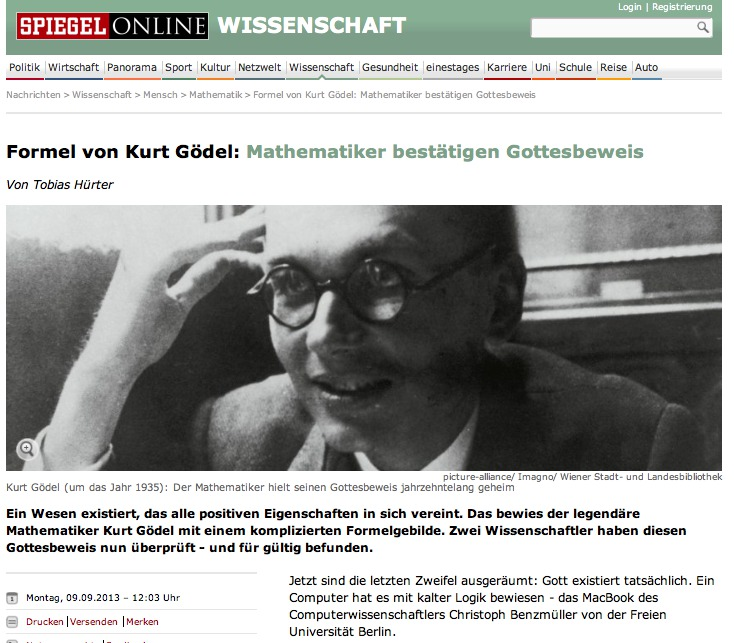
\includegraphics[width=\textwidth]{Images/News/spiegel1}} 
\vskip1em
Germany \\
- Telepolis \& Heise \\
- Spiegel Online \\
- FAZ \\
- Die Welt \\
- Berliner Morgenpost \\
- Hamburger Abendpost \\

\end{minipage} \hfill
%
\begin{minipage}{.35\textwidth}
Austria \\
- Die Presse \\
- Wiener Zeitung \\
- ORF \\

International \\
- Spiegel International \\
- Yahoo Finance \\
% - CNET \\
- United Press Intl. \\

India \\
- DNA India \\
- Delhi Daily News \\
- India Today \\

US \\
- ABC News \\

Italy \\
- Repubblica \\

Spain, Russia, Brazil, Bulgaria \\

\ldots

\end{minipage}
\end{frame}



\begin{frame}{A Long History}{\textcolor{blue}{pros} and \textcolor{red}{cons}} \Large

\hskip-.5em
\ldots\rotatebox[origin = bl,width = 0mm]{65}{\textcolor{blue}{Anselm v. C.}} \hskip-2.3em
          \rotatebox[origin = bl]{65}{\textcolor{red}{Gaunilo}} \hskip-1.3em
\ldots  \rotatebox[origin = bl]{65}{\textcolor{red}{Th. Aquinas}}  \hskip-2.3em
\ldots\ldots   \rotatebox[origin = bl]{65}{\textcolor{blue}{Descartes}} \hskip-1.7em
               \rotatebox[origin = bl]{65}{\textcolor{blue}{Spinoza}} \hskip-1.3em
               \rotatebox[origin = bl]{65}{\textcolor{blue}{Leibniz}}  \hskip-1.2em
\ldots  \rotatebox[origin = bl]{65}{\textcolor{red}{Hume}}  \hskip-1em
          \rotatebox[origin = bl]{65}{\textcolor{red}{Kant}}  \hskip-.8em
\ldots  \rotatebox[origin = bl]{65}{\textcolor{blue}{Hegel}}  \hskip-1.3em
\ldots  \rotatebox[origin = bl]{65}{\textcolor{red}{Frege}}  \hskip-1.3em
\ldots  \rotatebox[origin = bl]{65}{\textcolor{blue}{Hartshorne}} \hskip-1.9em
          \rotatebox[origin = bl]{65}{\textcolor{blue}{Malcolm}}  \hskip-1.4em
          \rotatebox[origin = bl]{65}{\textcolor{red}{Lewis}}  \hskip-1em
          \rotatebox[origin = bl]{65}{\textcolor{blue}{Plantinga}}  \hskip-1.6em
          \rotatebox[origin = bl]{65}{\textcolor{blue}{G\"odel}}   \hskip-1.2em
\ldots \\[1em]

\pause
\vfill
Anselm's notion of God:\\
\,\hfill \emph{``God is that, than which nothing greater can be
  conceived.''} \\[1em]

G\"odel's notion of God:\\
\,\hfill \emph{``A God-like being possesses all `positive' properties.''} \\[1em]

To show by logical reasoning: \\
\,\hfill \emph{``(Necessarily) God exists.''} \\[1em]

\end{frame}



\begin{frame}{The Ontological Proof Today}
\vskip1em
\emph{\huge Wohl eine jede Philosophie kreist um den ontologischen
  Gottesbeweis} \\[1.5em]
(Adorno, Th. W.: Negative Dialektik. Frankfurt a. M. 1966, p.378)
\vfill
\begin{center}
\fcolorbox{gray}{white}{
\begin{minipage}{0.9\textwidth}
\hfill
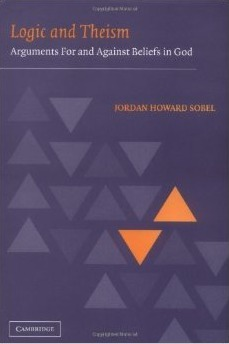
\includegraphics[height=2.2cm]{Images/Books/buch3.jpg} \hfill

\includegraphics[height=2.2cm]{Images/Books/buch2.jpg} \hfill 
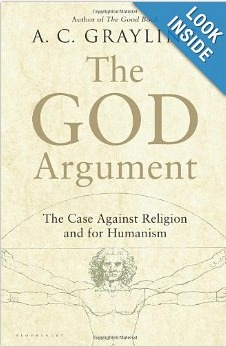
\includegraphics[height=2.2cm]{Images/Books/buch4.jpg} \hfill
\hfill

\vspace{0.5 cm}

\hfill
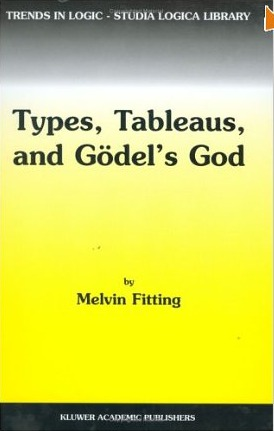
\includegraphics[height=2.2cm]{Images/Books/buch7.jpg} \hfill
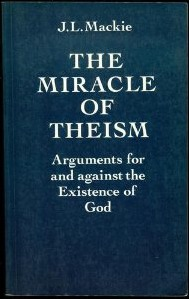
\includegraphics[height=2.2cm]{Images/Books/buch5.jpg} \hfill
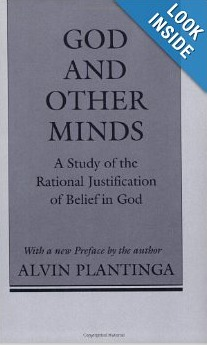
\includegraphics[height=2.2cm]{Images/Books/buch6.jpg} \hfill

\includegraphics[height=2.2cm]{Images/Books/buch1.jpg} \hfill
\hfill
\end{minipage}
}

\end{center}
\end{frame}


\begin{frame}{Motivations} \Large
\begin{itemize}
\item \textcolor{blue}{Philosophical:} 
  \begin{itemize}
  \item Limits of metaphysics \& epistemology
  \item \emph{Metaphysical} versus \emph{logical} necessary existence \\[2em]
  \end{itemize} 
\item \textcolor{blue}{Theological:} 
  \begin{itemize}
  \item Investigations of the nature of God
  \item Arguments to convince atheists \\[2em]
  \end{itemize}
\item \textcolor{red}{Computational:} can automated reasoners be used \ldots
  \begin{itemize}
  \item \ldots to formalize the definitions, axioms and theorems?
  \item \ldots to verify the arguments step-by-step?
  \item \ldots to fully automate (sub-)arguments? \\[2em]
  \end{itemize}
\end{itemize}

\begin{center}
  \textcolor{red}{\emph{``Computer-assisted Theoretical Philosophy''}}
\end{center}
\end{frame}
